\documentclass{article}

\usepackage[preprint]{neurips_2026}

\usepackage[utf8]{inputenc}
\usepackage[T1]{fontenc}
\usepackage{hyperref}
\usepackage{url}
\usepackage{booktabs}
\usepackage{amsfonts}
\usepackage{amsmath}
\usepackage{nicefrac}
\usepackage{microtype}
\usepackage{xcolor}
\usepackage{graphicx}
\usepackage{tikz}
\usetikzlibrary{positioning,arrows.meta,calc,fit,backgrounds}
\usepackage{float}
\newcommand{\TODO}[1]{\textcolor{red}{[TODO: #1]}}

\title{Detecting Vulnerable C Functions from Token Sequences with Fine-Tuned Code Transformers}

\author{%
  Kareem Rammah \\
  University of Toronto Mississauga \\
  \texttt{kareem.rammah@mail.utoronto.ca} \\
  \And
  Danny Leo \\
  University of Toronto Mississauga \\
  \texttt{d.leo@mail.utoronto.ca} \\
}

\begin{document}

\maketitle

\begin{abstract}
Security vulnerabilities in widely used C software are slow to find by manual code review. Examples are writing past the end of a memory buffer and using memory after it has been freed. This motivates automated detection.
We study function-level vulnerability detection. Given the source code of one C function, a model predicts whether the function contains a security vulnerability.
We treat the function as a variable-length sequence of subword tokens and compare two sequence models.
The baseline is a bidirectional long short-term memory (LSTM) network trained from scratch.
The second model is CodeBERT, a Transformer encoder pre-trained on source code, which we fine-tune for binary classification.
We use the Devign dataset from the CodeXGLUE benchmark. It contains 27{,}318 functions from two open-source C projects, the multimedia library FFmpeg and the machine emulator QEMU. Each function is labelled as vulnerable or not.
We report accuracy, precision, recall, F1, and ROC-AUC on the held-out test split, averaged over three random seeds. We also run ablations on input truncation, the number of fine-tuned layers, and pre-trained embeddings for the BiLSTM.
The BiLSTM reaches 64.8\% accuracy. CodeBERT reaches 65.3\% at one learning rate and 62.3\% at another, so its result depends more on the learning rate than on the choice between the two models. We find no clear benefit from pre-training.
Both models match or exceed the published 59.4\% and 62.1\%.
Accuracy falls as functions get longer, and on average the models miss 30\% to 41\% of vulnerable functions at the default threshold, with up to 50\% for individual seeds.
We also find that about 5\% of vulnerable functions, and almost no non-vulnerable ones, end without a closing brace. The models classify these functions much more accurately than the rest, which suggests that they exploit this formatting artifact.
\end{abstract}

\section{Introduction}

\textbf{Motivation:}
Memory safety and input validation bugs in C programs are a common source of security incidents. They are expensive to find, because reading code manually takes time and expertise.
Static analysis tools based on hand-written rules can produce many false alarms. They can also miss vulnerability patterns that their authors did not anticipate.
Learning-based detectors learn patterns from labelled examples of vulnerable and non-vulnerable code. They could be used to prioritize which functions human reviewers inspect first.

\textbf{Task:}
The input to our model is the source text of one C function. We tokenize it into a sequence of $n$ subword tokens $x_1,\dots,x_n$, where $n$ ranges from a few tokens to thousands.
The output is a single probability $\hat{y}\in[0,1]$ that the function is vulnerable.
This is a sequence classification problem. Recurrent and Transformer models are natural choices, because both accept variable-length input and both can capture long-range dependencies. One example is a buffer allocated at the top of a function and misused many lines later.

\textbf{Approach:}
We compare a bidirectional LSTM trained from scratch with a fine-tuned CodeBERT model.
Fine-tuning a model pre-trained on millions of functions is reasonable because the labelled data is small compared with the diversity of C code. Representations learned from large unlabelled data may transfer.
It is unclear how large the benefit of pre-training is on this task. On this benchmark, CodeBERT reaches 62.08\% accuracy against 59.37\% for a BiLSTM~\citep{lu2021codexglue}. Measuring this gap carefully is an important question in our project.
If the gap is small, pre-training adds little when the input is a flat token sequence. This would suggest that label noise, truncation, or dataset-specific signal limits both models more than representation quality does.
If the gap is large, transfer from code pre-training matters even without parsers or graphs. This would support its use where labelled vulnerabilities are scarce.

\textbf{Contributions:}
We make three contributions. First, we release a reproducible pipeline for training and evaluating both models on a single fixed split. Second, we quantify the gain from pre-training over a recurrent baseline with multiple random seeds. Third, we analyze errors by function length and by manual inspection of confidently misclassified functions.
Under identical tokenization and splits, the two models performed within seed-to-seed variation of each other. Both degraded on long functions. We also document a formatting artifact in the dataset.

\section{Background and Related Work}

\textbf{Background:}
A \emph{recurrent neural network} reads tokens one at a time and keeps a hidden state. A long short-term memory network (LSTM)~\citep{hochreiter1997lstm} adds gates that help preserve information over long sequences. A \emph{bidirectional} LSTM (BiLSTM) reads the sequence in both directions.
A \emph{Transformer} encoder~\citep{vaswani2017attention} replaces recurrence with self-attention, so every token can attend to every other token.
CodeBERT~\citep{feng2020codebert} is a Transformer encoder with the RoBERTa architecture~\citep{liu2019roberta}, a refined version of the BERT encoder. It is pre-trained on pairs of natural language and code in six programming languages. It prepends a special \texttt{[CLS]} token whose final hidden state summarizes the whole input.
\emph{Fine-tuning} continues training the pre-trained weights, together with a small new output layer, on the downstream task.

\textbf{Deep learning for vulnerability detection:}
\citet{zhou2019devign} introduced the dataset used here. They proposed a gated graph neural network, which passes information along the edges of a graph. The graph joins three views of each function. These are the abstract syntax tree (the grammatical structure of the code), the control flow (the order in which statements may execute), and the data flow (how values move between variables). On their own four-project data, they report an average accuracy gain of 10.51\% over the methods of the time.
The CodeXGLUE benchmark~\citep{lu2021codexglue} later packaged the FFmpeg and QEMU portion of this data. It reports test accuracies of 59.37\% for a BiLSTM and 62.08\% for CodeBERT~\citep{feng2020codebert}. GraphCodeBERT~\citep{guo2021graphcodebert} reaches 62.30\% in the evaluation of \citet{nguyen2022regvd}.
ReGVD~\citep{nguyen2022regvd} avoids expensive program analysis. It builds a graph directly from the token sequence and applies a graph neural network with residual connections. Its best accuracy is 63.69\%, which is 1.61 percentage points above CodeBERT.

A recent study by \citet{labtoreality2025} trains Devign, ReVeal, LineVul, and VulBERTa on four datasets, including Devign. The models generalize poorly across datasets. ReVeal and LineVul perform sharply worse on a newly collected set of 200 recent Linux and Chromium vulnerabilities. This motivates our error analysis, since a model trained on Devign may learn dataset-specific patterns rather than vulnerability semantics.

\textbf{Our contribution relative to prior work:}
We do not propose a new architecture. We study the simplest strong sequence-only setting, with no parsers and no graphs. We compare a recurrent model trained from scratch with a fine-tuned pre-trained Transformer under the same tokenization, splits, and seeds. We also analyze failures by function length and truncation.

\section{Data}\label{sec:data}

\textbf{Source:}
We use the Devign vulnerability dataset~\citep{zhou2019devign} in the form released with CodeXGLUE~\citep{lu2021codexglue}.
Each example is the raw text of one C function from FFmpeg (a multimedia processing library) or QEMU (a machine emulator), with a binary label (1 = vulnerable).
The functions were taken from security-related commits and manually labelled as vulnerable or not~\citep{zhou2019devign}. The original Devign study used four projects. The released benchmark contains the FFmpeg and QEMU portion.
The data is available in the Hugging Face \texttt{datasets} library and the CodeXGLUE repository.

\textbf{Size and split:}
The benchmark has 27{,}318 functions, split into 21{,}854 training, 2{,}732 validation, and 2{,}732 test examples.
The fraction of vulnerable examples is 45.8\%, 43.4\%, and 45.9\% in the three splits (Figure~\ref{fig:eda}, left). The classes are close to balanced, so accuracy is a meaningful metric alongside F1.
We use the fixed split provided by the benchmark, so that our numbers can be compared with published results.

\begin{figure}[h!]
  \centering
  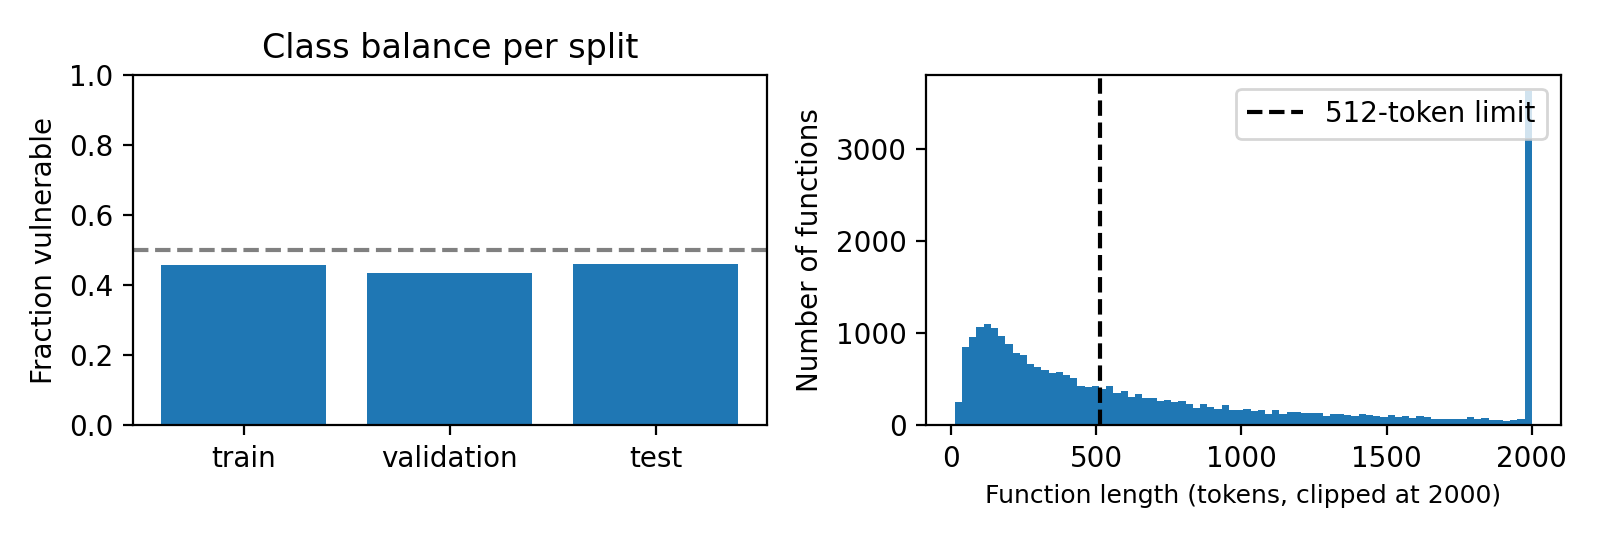
\includegraphics[width=\linewidth]{eda.png}
  \caption{Exploratory statistics of the Devign/CodeXGLUE data. The left panel shows the fraction of vulnerable functions in the training, validation, and test splits, which is between 43\% and 46\% in each. The right panel shows the distribution of function length in subword tokens. Functions longer than 2{,}000 tokens are grouped into the last bar, and the dashed line marks CodeBERT's 512-token input limit. Almost half of all functions go past this limit.}
  \label{fig:eda}
\end{figure}

\textbf{Exploratory analysis:}
Function length is heavy-tailed (Figure~\ref{fig:eda}, right). In CodeBERT's tokenization, the median function has 482 tokens, the mean is 1{,}114, and the 90th percentile is 2{,}420. The longest function has 90{,}858 tokens. These counts are made after deduplication and exclude \texttt{[CLS]} and \texttt{[SEP]}.
Because 48.1\% of functions exceed the 512-token input limit, truncation discards code for about half of the data. The discarded code might contain the vulnerable lines.
Vulnerable functions tend to be a little longer than non-vulnerable ones (training medians of 522 and 443 tokens), so a model could exploit length as a shortcut. We therefore include a length-only classifier as a trivial reference.

The most frequent tokens are almost the same in the two classes. They are underscores, line breaks, punctuation, and operators such as \texttt{->}. No obvious word or character separates the classes, which suggests that detection requires context and not keyword counting.
An exact-match check, after normalizing whitespace, finds 10 test and 8 validation functions that also appear in the training set. Only 21{,}796 of the 21{,}854 training examples are unique. These overlaps are small, but they would slightly raise the scores if they were left in.

\textbf{A formatting artifact:}
Some functions end without a closing brace. This holds for 5.8\% of vulnerable training functions but for under 0.1\% of non-vulnerable ones (5.2\% and under 0.1\% in the test split). In the test split, 65 of the 2{,}732 functions (2.4\%) lack a final brace, and all 65 are vulnerable.
The three models classify these functions with 89\% to 93\% accuracy, against 62\% to 65\% on the rest. Excluding them lowers overall accuracy by only 0.6 to 0.7 points (BiLSTM 64.8\% to 64.1\%, CodeBERT at $2\times10^{-5}$ 65.3\% to 64.7\%, CodeBERT at $3\times10^{-5}$ 62.3\% to 61.6\%). This is too little to explain the gap to published results, but part of the signal is not about vulnerabilities. We keep these functions to stay comparable with published results.

\textbf{Preprocessing:}
Functions are tokenized with CodeBERT's byte-level byte-pair encoding (BPE) tokenizer. It splits text into frequent subword pieces. We use it for both models, so that differences in performance come from the model and not from the vocabulary.
We remove duplicate training functions and any training function that also appears in the validation or test split. This leaves 21{,}778 training functions.
Inputs are truncated to a maximum length $L$ (default 512 tokens, counting the special tokens) and padded within each batch. We do not strip comments or rename identifiers.
Many functions exceed the limit, so we compare keeping the first $L$ tokens (\emph{head}) with keeping the first and last $L/2$ tokens (\emph{head+tail}).
No feature normalization is needed, because the inputs are token identifiers. The preprocessing code and random seeds are in the project repository.

\section{Model Architecture}

Both models share the same input and output (Figure~\ref{fig:arch}).
A function is tokenized to $x_{1:n}$, truncated to $L$ tokens, and mapped to a probability $\hat{y}=\sigma(\mathbf{w}^\top \mathbf{h} + b)$, where $\mathbf{h}\in\mathbb{R}^d$ is a summary vector of the function.
Training minimizes the binary cross-entropy $\mathcal{L}=-\big[y\log\hat{y}+(1-y)\log(1-\hat{y})\big]$.

\begin{figure}[h!]
  \centering
  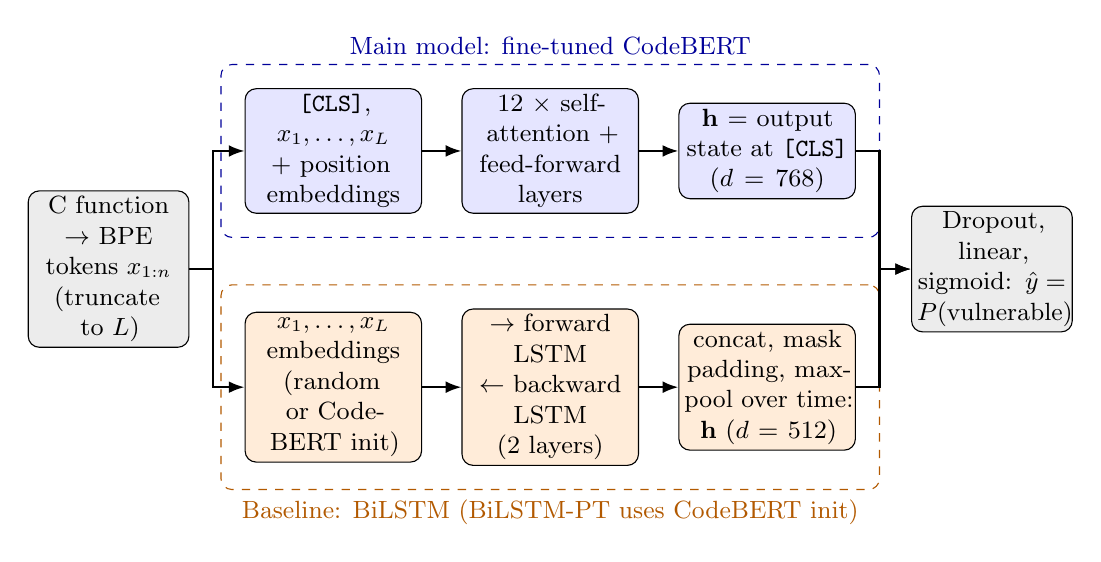
\begin{tikzpicture}[
      node distance=5mm,
      box/.style={draw, rounded corners, align=center, minimum height=11mm, text width=2.1cm, font=\small, inner sep=2pt},
      main/.style={box, fill=blue!10},
      base/.style={box, fill=orange!15},
      io/.style={box, fill=gray!15, text width=1.9cm},
      arr/.style={-{Latex[length=2mm]}, thick},
      grp/.style={draw, rounded corners, dashed, inner sep=3mm}
    ]
    \node[io] (tok) {C function $\to$ BPE tokens $x_{1:n}$ (truncate to $L$)};

    \node[main, right=7mm of tok, yshift=15mm] (m1) {\texttt{[CLS]}, $x_1,\dots,x_L$ + position embeddings};
    \node[main, right=of m1] (m2) {12 $\times$ self-attention + feed-forward layers};
    \node[main, right=of m2] (m3) {$\mathbf{h}=$ output state at \texttt{[CLS]} ($d=768$)};

    \node[base, right=7mm of tok, yshift=-15mm] (b1) {$x_1,\dots,x_L$ embeddings (random or CodeBERT init)};
    \node[base, right=of b1] (b2) {$\rightarrow$ forward LSTM\\$\leftarrow$ backward LSTM\\(2 layers)};
    \node[base, right=of b2] (b3) {concat, mask padding, max-pool over time: $\mathbf{h}$ ($d=512$)};

    \node[io, anchor=west] (out) at ($(m3.east)!0.5!(b3.east)+(7mm,0)$) {Dropout, linear, sigmoid: $\hat{y}=P(\text{vulnerable})$};

    \draw[arr] (tok.east) -- ++(3mm,0) |- (m1.west);
    \draw[arr] (tok.east) -- ++(3mm,0) |- (b1.west);
    \draw[arr] (m1) -- (m2);
    \draw[arr] (m2) -- (m3);
    \draw[arr] (b1) -- (b2);
    \draw[arr] (b2) -- (b3);
    \draw[arr] (m3.east) -- ++(3mm,0) |- (out.west);
    \draw[arr] (b3.east) -- ++(3mm,0) |- (out.west);

    \begin{scope}[on background layer]
      \node[grp, draw=blue!60!black, fit=(m1)(m2)(m3),
            label={[font=\small, text=blue!60!black]above:Main model: fine-tuned CodeBERT}] {};
      \node[grp, draw=orange!70!black, fit=(b1)(b2)(b3),
            label={[font=\small, text=orange!70!black]below:Baseline: BiLSTM (BiLSTM-PT uses CodeBERT init)}] {};
    \end{scope}
  \end{tikzpicture}
  \caption{Overview of the two compared models. A C function is tokenized once and given to either the fine-tuned CodeBERT encoder (top, blue) or the BiLSTM baseline (bottom, orange). CodeBERT takes the output state at the prepended \texttt{[CLS]} token as the summary vector $\mathbf{h}$. The BiLSTM concatenates its forward and backward states and takes the element-wise maximum over time, ignoring padded positions. A dropout and linear layer with a sigmoid converts $\mathbf{h}$ into the probability that the function is vulnerable. For the BiLSTM-PT variant, the embeddings are initialized from CodeBERT and passed through a learned linear projection to 256 dimensions.}
  \label{fig:arch}
\end{figure}

\textbf{Baseline: BiLSTM:}
Token identifiers are mapped to 256-dimensional learned embeddings. These hold about 12.9M parameters for the 50{,}265-token vocabulary, and the model has 15.5M parameters in total.
A two-layer bidirectional LSTM with 256 hidden units per direction processes the embeddings. Element-wise max-pooling over time gives $\mathbf{h}\in\mathbb{R}^{512}$. Max-pooling lets any position in a long function contribute a strong signal, without relying on the final hidden state to remember it.
Sequences are passed to the LSTM as packed padded sequences, so that padding tokens do not affect either direction. Padded positions are also masked before max-pooling, so that only real input tokens contribute to the function representation.

We use dropout 0.3 between layers and train with Adam from random initialization (learning rate $10^{-3}$, batch size 32, 10 epochs, gradient-norm clipping at 1.0). We select the checkpoint with the best validation F1, as for CodeBERT.

To separate the effect of pre-trained token embeddings from that of pre-trained contextual layers, we also train a BiLSTM-PT variant. Its embedding layer is initialized from CodeBERT's input token embeddings, and it is otherwise the same. CodeBERT's embeddings have 768 dimensions and the baseline uses 256, so we add a learned linear projection from 768 to 256 dimensions before the LSTM. The pre-trained embeddings remain trainable. This variant has 41.4M parameters.
The maximum length $L$ counts special tokens such as \texttt{[CLS]}. With $L = 512$, a function contributes at most 510 content tokens.

\textbf{Main model: fine-tuned CodeBERT:}
CodeBERT has 125M parameters, 12 layers, 12 attention heads, and hidden size 768. It embeds each token and adds position embeddings. Self-attention layers then let every token attend to all others, so that a use of a variable can be related to its declaration anywhere in the function.
We take the final hidden state of the \texttt{[CLS]} token as $\mathbf{h}$, apply dropout 0.1, and add a single linear layer to produce a logit.
We fine-tune all weights with AdamW, which is Adam with decoupled weight decay. The learning rate is $2\times10^{-5}$ and the weight decay is 0.01. We warm up linearly over the first 10\% of steps and then decay linearly. The batch size is 16, training lasts 5 epochs, gradient norms are clipped at 1.0, and we use mixed precision. We keep the checkpoint with the best validation F1.
All models are implemented in PyTorch~\citep{paszke2019pytorch} with the Hugging Face Transformers library~\citep{wolf2020transformers}. Experiments ran on a single NVIDIA Tesla T4 GPU in Google Colab. One CodeBERT run took about 50 minutes and one BiLSTM run about 11 minutes.

\textbf{Hyperparameter tuning:}
We tuned only the learning rate, on seed 0, by best validation F1. For the BiLSTM, $5\times10^{-4}$, $10^{-3}$, and $2\times10^{-3}$ gave 0.609, 0.632, and 0.616, so we kept $10^{-3}$.
For CodeBERT, $10^{-5}$, $2\times10^{-5}$, and $3\times10^{-5}$ gave 0.578, 0.618, and 0.639. The two larger rates had the same best validation ROC-AUC (0.739).
Because $3\times10^{-5}$ had the highest validation F1, we also ran seeds 1 and 2 with it and report both settings in Table~\ref{tab:main}. On the test set it gave lower accuracy and ROC-AUC. The ablations used $2\times10^{-5}$. We did not tune batch size, dropout, or the number of epochs.
Repeating a configuration with the same seed gave different results (best validation F1 of 0.566 and 0.578 for $10^{-5}$), because GPU kernels are not deterministic. Differences of about one point of validation F1 are therefore within noise.

\textbf{Evaluation and ablations:}
We report accuracy, precision, recall, F1, and ROC-AUC on the test split with a decision threshold of 0.5. Precision is the fraction of functions flagged as vulnerable that truly are. Recall is the fraction of vulnerable functions that are flagged. F1 is their harmonic mean. ROC-AUC is the probability that a randomly chosen vulnerable function receives a higher score than a randomly chosen non-vulnerable one.
Results are averaged over three random seeds, with standard deviations, and compared against a length-only logistic regression.
The ablations vary three things. The first is the truncation length $L \in \{128, 256, 512\}$ and strategy (first $L$ tokens versus first and last $L/2$). The second is the number of CodeBERT layers that are fine-tuned (top 4 versus all 12). The third is random versus CodeBERT-initialized BiLSTM embeddings (BiLSTM-PT).
For error analysis, we break down accuracy by function length and inspect confidently wrong predictions.

\section{Results}

Accuracy suits the near-balanced classes (45.9\% vulnerable in the test split) and allows comparison with published work. F1 balances precision and recall. ROC-AUC does not depend on the 0.5 threshold. Recall matters most for deployment, since a missed vulnerability is the costly error.
Table~\ref{tab:main} compares the models on the test split. Table~\ref{tab:abl} reports the ablations, Table~\ref{tab:len} breaks accuracy down by function length, and Figure~\ref{fig:curves} shows training curves.

\begin{table}[h!]
  \caption{Test-set results in \% (mean $\pm$ population standard deviation over three seeds). The length-only classifier is a logistic regression on the log token count (one run). CodeBERT is shown at two learning rates.}
  \label{tab:main}
  \centering
  \small
  \begin{tabular}{lccccc}
    \toprule
    Model & Accuracy & Precision & Recall & F1 & ROC-AUC \\
    \midrule
    Length-only LR & 52.5 & 41.1 & 7.7 & 13.0 & 50.5 \\
    BiLSTM (baseline) & 64.8 $\pm$ 0.5 & 61.6 $\pm$ 2.2 & 63.5 $\pm$ 6.8 & 62.2 $\pm$ 2.3 & 72.2 $\pm$ 0.6 \\
    CodeBERT, lr $2\times10^{-5}$ & 65.3 $\pm$ 1.8 & 64.0 $\pm$ 4.6 & 59.1 $\pm$ 8.2 & 60.8 $\pm$ 2.1 & 72.6 $\pm$ 1.3 \\
    CodeBERT, lr $3\times10^{-5}$ & 62.3 $\pm$ 2.4 & 57.7 $\pm$ 3.3 & 70.3 $\pm$ 5.8 & 63.1 $\pm$ 1.2 & 70.7 $\pm$ 2.2 \\
    \bottomrule
  \end{tabular}
\end{table}

\begin{table}[h!]
  \caption{Ablations on the test set in \%. All rows use seed 0. The first row of each model is its seed-0 reference, which is the fair comparison point, because CodeBERT's seed 0 was its weakest seed.}
  \label{tab:abl}
  \centering
  \small
  \begin{tabular}{llccc}
    \toprule
    Model & Variant & Accuracy & F1 & ROC-AUC \\
    \midrule
    CodeBERT & $L=512$, first tokens (reference) & 62.7 & 63.3 & 70.7 \\
    CodeBERT & $L=256$ & 62.4 & 63.5 & 70.4 \\
    CodeBERT & $L=128$ & 61.5 & 60.8 & 68.4 \\
    CodeBERT & first and last $L/2$ tokens & 66.1 & 60.9 & 74.0 \\
    CodeBERT & top 4 layers fine-tuned & 64.4 & 59.3 & 70.3 \\
    \midrule
    BiLSTM & $L=512$, first tokens (reference) & 64.2 & 64.6 & 71.5 \\
    BiLSTM & first and last $L/2$ tokens & 64.0 & 59.8 & 72.3 \\
    BiLSTM-PT & CodeBERT embedding init & 62.2 & 60.5 & 69.4 \\
    \bottomrule
  \end{tabular}
\end{table}

\begin{table}[h!]
  \caption{Test accuracy (\%) by function length in subword tokens, averaged over three seeds ($n$ is the number of test functions). CodeBERT is at $2\times10^{-5}$.}
  \label{tab:len}
  \centering
  \small
  \begin{tabular}{lcccccc}
    \toprule
    Length & $<$128 & 128--256 & 256--512 & 512--1k & 1k--2k & $>$2k \\
    \midrule
    $n$ & 357 & 480 & 545 & 560 & 449 & 341 \\
    CodeBERT & 75.4 & 71.1 & 66.5 & 61.1 & 60.8 & 57.2 \\
    BiLSTM & 77.1 & 69.1 & 65.8 & 59.8 & 60.4 & 58.5 \\
    \bottomrule
  \end{tabular}
\end{table}

\begin{figure}[h!]
  \centering
  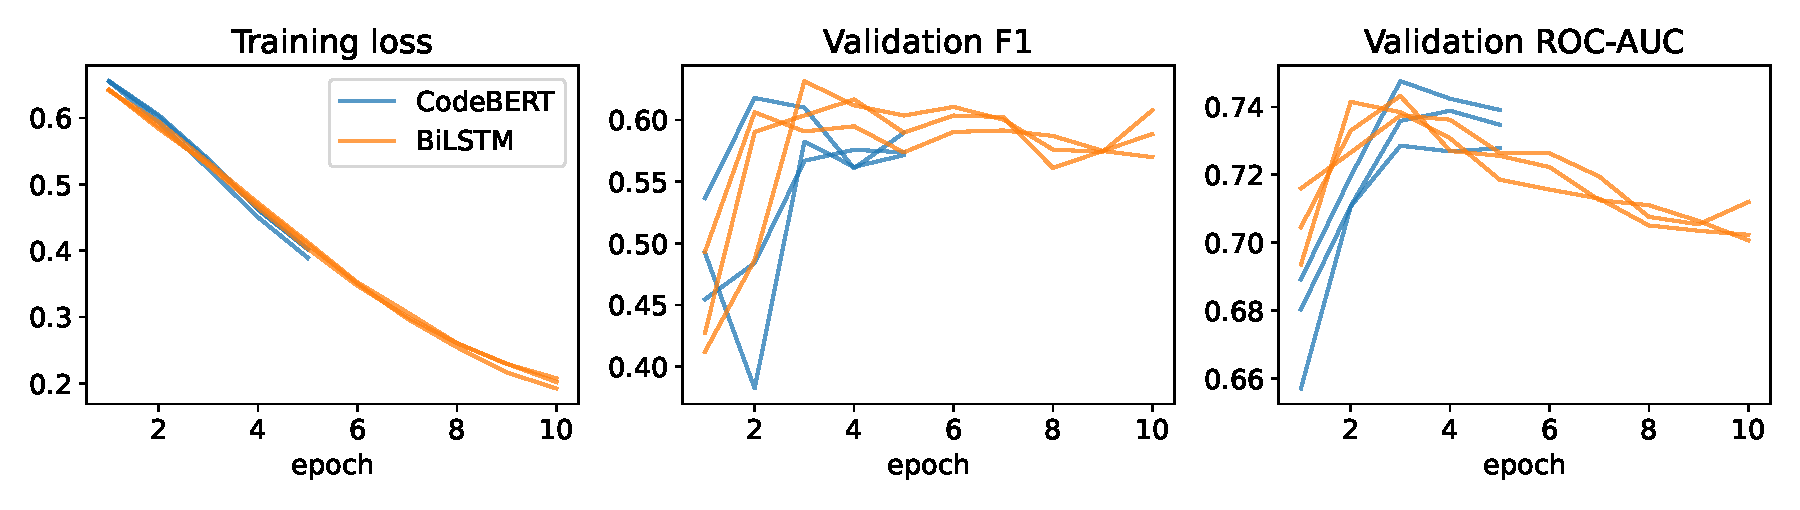
\includegraphics[width=\linewidth]{fig_curves.pdf}
  \caption{Training loss (left), validation F1 (middle), and validation ROC-AUC (right) per epoch for the BiLSTM (orange, 10 epochs) and CodeBERT (blue, 5 epochs), with one thin line per seed. Training loss keeps falling, while the BiLSTM's validation ROC-AUC peaks after about 3 to 4 epochs and then declines.}
  \label{fig:curves}
\end{figure}

The length-only classifier reaches 52.5\% accuracy. This is below the 54.1\% obtained by always predicting non-vulnerable, and its recall is only 7.7\%.
The BiLSTM and CodeBERT ($2\times10^{-5}$) reach 64.8\% and 65.3\% accuracy. Across seeds, accuracy ranges from 64.2\% to 65.3\% for the BiLSTM and from 62.7\% to 66.7\% for CodeBERT.
At $3\times10^{-5}$, CodeBERT reaches 62.3\% accuracy and 70.7\% ROC-AUC, but it has the highest recall (70.3\%) and F1 (63.1\%) of the three models. Its per-seed accuracies are 60.9\%, 60.3\%, and 65.7\%.
Precision and recall vary more between seeds than accuracy does. At $2\times10^{-5}$, CodeBERT's recall ranges from 50.4\% to 70.0\%.
At the 0.5 threshold, the models miss many vulnerable functions. On average, the false-negative rate (100\% minus recall) is 36.5\% for the BiLSTM and 40.9\% and 29.7\% for CodeBERT at $2\times10^{-5}$ and $3\times10^{-5}$. For individual seeds, it is 30.0\%, 49.6\%, and 43.1\% for CodeBERT ($2\times10^{-5}$) and 29.1\%, 35.1\%, and 45.5\% for the BiLSTM.

\section{Discussion}

\textbf{Pre-training:}
We find no clear benefit from pre-training. At the learning rate $2\times10^{-5}$, CodeBERT's mean accuracy and ROC-AUC exceed the BiLSTM's by 0.5 and 0.4 points. This is less than CodeBERT's own spread over three seeds (1.8 and 1.3 points).
At $3\times10^{-5}$, CodeBERT is 2.5 points lower in accuracy and 1.5 points lower in ROC-AUC, but higher in F1 (63.1\% against 62.2\%) and recall (70.3\% against 63.5\%). Changing the learning rate moves CodeBERT's accuracy by 3 points, which is more than the gap between the two architectures.
With three seeds, we cannot separate the models, and we cannot claim that they are equal.

This matches the ``small gap'' case in our proposal. On a flat token sequence, a recurrent model trained from scratch does about as well as a fine-tuned pre-trained Transformer. This suggests that label noise, truncation, or dataset-specific signal limits both models more than representation quality does.

\textbf{Comparison with published results:}
When CodeBERT uses its better learning rate, both models exceed the published figures. The BiLSTM reaches 64.8\% against 59.4\%, and CodeBERT reaches 65.3\% against 62.1\%. The BiLSTM gains more. At $3\times10^{-5}$, CodeBERT only matches its published number (62.3\% against 62.1\%).
We did not reproduce the published training setup. Our tokenizer, input length, pooling, and checkpoint selection may differ from it, so we cannot say why. We selected models on validation data only and used the test set once.

\textbf{Pre-trained embeddings:}
Initializing the BiLSTM with CodeBERT's embeddings did not help either. Test accuracy was 62.2\% against 64.2\% for the seed-0 reference, and validation ROC-AUC was 0.715 against 0.738. The benefit of CodeBERT is therefore not located in its token embeddings.

\textbf{Overfitting and variance:}
Both models overfit. The BiLSTM's training loss falls from 0.64 to about 0.25 by epoch 8, while its validation ROC-AUC peaks around epoch 3 and then declines. CodeBERT's validation ROC-AUC flattens after epoch 3 to 4 (Figure~\ref{fig:curves}).
The seed-to-seed variance in precision and recall is large. Part of it comes from selecting checkpoints by validation F1 at a fixed 0.5 threshold, which can pick under-trained checkpoints. At $2\times10^{-5}$, seed 0 selected epoch 2 (validation F1 0.618, ROC-AUC 0.711), although epoch 4 had a higher ROC-AUC (0.739). Seed 0 is also CodeBERT's weakest seed at this learning rate.
At $3\times10^{-5}$, the rule selected epoch 1 for seed 1. That checkpoint has a validation ROC-AUC of 0.688, while epoch 3 of the same run reached 0.746. This probably explains the low test results at this learning rate (60.9\%, 60.3\%, and 65.7\% accuracy). Selecting by ROC-AUC would likely avoid this, but we did not run it, so the explanation is untested.

\textbf{Truncation and input length:}
Shortening CodeBERT's input from 512 to 256 tokens left seed-0 accuracy unchanged (62.4\% against 62.7\%). The 128-token input was slightly lower (61.5\%, ROC-AUC 68.4 against 70.7). We see no evidence that extra context matters much on its own.
Keeping the first and last $L/2$ tokens gave a higher ROC-AUC than keeping the first $L$ tokens, for both models and on both the validation and test splits. For CodeBERT, validation ROC-AUC was 0.750 against 0.739 and test ROC-AUC 74.0 against 70.7. For the BiLSTM, the values were 0.759 against 0.738 and 72.3 against 71.5. Accuracy did not change consistently. Each difference comes from one seed and is about the size of the seed variation, so we treat it as suggestive only.
Fine-tuning only the top four layers (28.9M trainable parameters, about 5.4 instead of 9.6 minutes per epoch) matched full fine-tuning within noise (64.4\% against 62.7\%).

\textbf{Function length:}
Accuracy falls with function length for both models (Table~\ref{tab:len}). For CodeBERT it drops from 75.4\% below 128 tokens to 57.2\% above 2{,}000 tokens. For the BiLSTM it drops from 77.1\% to 58.5\%. The longest bucket is only 3 to 4 points above the 54.1\% majority-class rate, so on the longest functions both models add little.
The decline is already visible among functions shorter than the 510-token limit (75.4\%, 71.1\%, and 66.5\% for CodeBERT across the first three buckets). Truncation therefore cannot be the only cause. A plausible additional reason is that the vulnerable lines are a smaller fraction of a longer function.

\textbf{Qualitative errors:}
We read 18 of CodeBERT's 20 most confident test errors in full and a 19th in part (seed 0). Fourteen are false positives and five are false negatives. The false positives are also more extreme: they reach a probability of 0.99, while the most confident false negatives stop at 0.17.
The false positives are non-vulnerable functions with low-level patterns, such as pointer arithmetic (\texttt{*dest++}), manual temporary allocation and release (\texttt{tcg\_temp\_new}, \texttt{tcg\_temp\_free}), inline assembly, and \texttt{\#if} guards. Judging by function names, ten of the fourteen come from QEMU, mostly CPU and device emulation code, and several use an older style (global \texttt{env} and \texttt{T0}), so the model may be reacting to style rather than to a defect.
The false negatives are short functions (31 to 192 tokens) that look correct in isolation, such as one that only returns \texttt{nb\_fds < shared}. Their labels probably reflect the surrounding commit or code outside the function, which is the label noise that our proposal anticipated.

We also read 15 of the BiLSTM's 20 most confident errors in full and a 16th in part (seed 0). Ten are false negatives and six are false positives, the reverse of CodeBERT's mix. Three false negatives are shared with CodeBERT. The others are mostly short functions that call other routines or take locks, so their defects, if any, depend on outside context. In \texttt{check\_checksum}, the checksum comparison is commented out and the function always returns 0, which appears to disable the check. The BiLSTM gave it a vulnerability probability of 0.114.
The BiLSTM's false positives are ordinary-looking QEMU block, KVM, vhost, and migration functions and FFmpeg H.264 code. None overlaps with CodeBERT's confident false positives.

One correct prediction is also instructive. CodeBERT labelled a function as vulnerable with probability 1.000, and the function is missing its closing braces. This matches the artifact in Section~\ref{sec:data}, where all three models classify functions without a final brace with 89\% to 93\% accuracy. Formatting may therefore explain such predictions.

\section{Limitations}

We expect the approach to perform worst on long functions, where truncation can remove the lines that contain the vulnerability. We also expect it to perform worse on code from other projects or authors. Only FFmpeg and QEMU are used, and \citet{labtoreality2025} report poor cross-dataset generalization.
Labels derive from security-fix commits and are noisy. They apply to whole functions, so a model cannot localize the faulty line. The models see only token text. They do not see types, macros, or other functions, which many real vulnerabilities depend on. The dataset also contains a formatting artifact (Section~\ref{sec:data}) that a model can exploit.
Our experiments also have limits. The ablations used a single seed, so differences of about two points are within seed noise. Only the learning rate was tuned, over three values. Selecting checkpoints by validation F1 added variance, and GPU non-determinism made identical configurations differ.
Possible extensions include sliding-window or hierarchical encoding of long functions, models with longer context, line-level supervision, selecting checkpoints by ROC-AUC, and evaluation on additional datasets.

\section{Ethical Considerations}

\textbf{Data:}
The data consists of public open-source code, but it is distributed under the licenses of the original projects. We share only code and a pointer to the source dataset, not a copy.
Labels come from manual annotation of functions drawn from security-related commits, so they may contain noise. A function changed in a security fix could be unrelated to the vulnerability, and an unchanged function could be vulnerable but unreported.
All examples come from two large projects maintained by experienced developers. The model may learn project-specific style rather than vulnerability semantics. Results should not be assumed to transfer to other codebases or to code written by less experienced programmers.

\textbf{Use and misuse:}
The most serious risk is false reassurance. A detector that misses real vulnerabilities (false negatives) may lead teams to skip human review. Our models miss 30\% to 41\% of vulnerable functions on average at the default threshold, and up to 50\% for individual seeds, so they are not a substitute for manual review.
A second risk is dual use. A model that ranks functions by likelihood of being vulnerable could also help an attacker decide where to look. The benefit may be larger for defenders, since the model is weak and attackers likely have stronger tools. This is our judgment rather than an established fact, so the risk remains.
We therefore present results as evidence about a research benchmark rather than a deployable scanner. We report false-negative rates explicitly and avoid releasing a polished tool.
Finally, flagged functions would be attributed to code written by specific developers. Any deployment should use the output to prioritize review and never as a measure of an individual's performance.

\section{Conclusion}

We compared a BiLSTM trained from scratch with fine-tuned CodeBERT for function-level vulnerability detection on Devign/CodeXGLUE, under identical tokenization and splits.
Over three seeds, the BiLSTM reached 64.8\% accuracy (72.2\% ROC-AUC). CodeBERT reached 65.3\% (72.6\%) at learning rate $2\times10^{-5}$ and 62.3\% (70.7\%) at $3\times10^{-5}$. The model difference is within seed variation and smaller than the effect of the learning rate, so pre-training gave no clear benefit here. Both models matched or exceeded the published numbers for this benchmark.
Both models overfit within a few epochs, lose accuracy as functions get longer, and miss 30\% to 41\% of vulnerable functions on average at a 0.5 threshold. The dataset also contains a formatting artifact that a model can exploit.
Natural next steps are selecting checkpoints by ROC-AUC, evaluating on other datasets, and encoding long functions without truncation.

\raggedright
\bibliographystyle{plainnat}
\begin{thebibliography}{99}

\bibitem[Feng et~al.(2020)]{feng2020codebert}
Zhangyin Feng, Daya Guo, Duyu Tang, Nan Duan, Xiaocheng Feng, Ming Gong, Linjun Shou, Bing Qin, Ting Liu, Daxin Jiang, and Ming Zhou.
\newblock CodeBERT: A pre-trained model for programming and natural languages.
\newblock In \emph{Findings of EMNLP}, 2020.

\bibitem[Guo et~al.(2021)]{guo2021graphcodebert}
Daya Guo, Shuo Ren, Shuai Lu, Zhangyin Feng, Duyu Tang, Shujie Liu, Long Zhou, Nan Duan, Alexey Svyatkovskiy, Shengyu Fu, Michele Tufano, Shao~Kun Deng, Colin Clement, Dawn Drain, Neel Sundaresan, Jian Yin, Daxin Jiang, and Ming Zhou.
\newblock GraphCodeBERT: Pre-training code representations with data flow.
\newblock In \emph{ICLR}, 2021.

\bibitem[Hochreiter and Schmidhuber(1997)]{hochreiter1997lstm}
Sepp Hochreiter and J{\"u}rgen Schmidhuber.
\newblock Long short-term memory.
\newblock \emph{Neural Computation}, 9(8):1735--1780, 1997.

\bibitem[Liu et~al.(2019)]{liu2019roberta}
Yinhan Liu, Myle Ott, Naman Goyal, Jingfei Du, Mandar Joshi, Danqi Chen, Omer Levy, Mike Lewis, Luke Zettlemoyer, and Veselin Stoyanov.
\newblock RoBERTa: A robustly optimized BERT pretraining approach.
\newblock \emph{arXiv preprint arXiv:1907.11692}, 2019.

\bibitem[Lu and Lagaisse(2025)]{labtoreality2025}
Chaomeng Lu and Bert Lagaisse.
\newblock From lab to reality: A practical evaluation of deep learning models and LLMs for vulnerability detection.
\newblock \emph{arXiv preprint arXiv:2512.10485}, 2025.

\bibitem[Lu et~al.(2021)]{lu2021codexglue}
Shuai Lu, Daya Guo, Shuo Ren, Junjie Huang, Alexey Svyatkovskiy, Ambrosio Blanco, Colin Clement, Dawn Drain, Daxin Jiang, Duyu Tang, Ge~Li, Lidong Zhou, Linjun Shou, Long Zhou, Michele Tufano, Ming Gong, Ming Zhou, Nan Duan, Neel Sundaresan, Shao~Kun Deng, Shengyu Fu, and Shujie Liu.
\newblock CodeXGLUE: A machine learning benchmark dataset for code understanding and generation.
\newblock In \emph{NeurIPS Datasets and Benchmarks}, 2021.

\bibitem[Nguyen et~al.(2022)]{nguyen2022regvd}
Van-Anh Nguyen, Dai~Quoc Nguyen, Van Nguyen, Trung Le, Quan~Hung Tran, and Dinh Phung.
\newblock ReGVD: Revisiting graph neural networks for vulnerability detection.
\newblock In \emph{ICSE Companion}, 2022.

\bibitem[Paszke et~al.(2019)]{paszke2019pytorch}
Adam Paszke et~al.
\newblock PyTorch: An imperative style, high-performance deep learning library.
\newblock In \emph{NeurIPS}, 2019.

\bibitem[Vaswani et~al.(2017)]{vaswani2017attention}
Ashish Vaswani, Noam Shazeer, Niki Parmar, Jakob Uszkoreit, Llion Jones, Aidan~N. Gomez, {\L}ukasz Kaiser, and Illia Polosukhin.
\newblock Attention is all you need.
\newblock In \emph{NeurIPS}, 2017.

\bibitem[Wolf et~al.(2020)]{wolf2020transformers}
Thomas Wolf et~al.
\newblock Transformers: State-of-the-art natural language processing.
\newblock In \emph{EMNLP: System Demonstrations}, 2020.

\bibitem[Zhou et~al.(2019)]{zhou2019devign}
Yaqin Zhou, Shangqing Liu, Jingkai Siow, Xiaoning Du, and Yang Liu.
\newblock Devign: Effective vulnerability identification by learning comprehensive program semantics via graph neural networks.
\newblock In \emph{NeurIPS}, 2019.

\end{thebibliography}

\end{document}
